% ============================================================================
%  fig_size_distribution.tex -- C2A test-set human-size distribution (real counts).
%  Counts from runs_sahi_tta baseline_640 per_size_gt_count (sqrt-area bins,
%  2,043 test images, 72,523 instances). Needs \usepackage{tikz} (+ amsmath).
%  Include with:  % ============================================================================
%  fig_size_distribution.tex -- C2A test-set human-size distribution (real counts).
%  Counts from runs_sahi_tta baseline_640 per_size_gt_count (sqrt-area bins,
%  2,043 test images, 72,523 instances). Needs \usepackage{tikz} (+ amsmath).
%  Include with:  % ============================================================================
%  fig_size_distribution.tex -- C2A test-set human-size distribution (real counts).
%  Counts from runs_sahi_tta baseline_640 per_size_gt_count (sqrt-area bins,
%  2,043 test images, 72,523 instances). Needs \usepackage{tikz} (+ amsmath).
%  Include with:  % ============================================================================
%  fig_size_distribution.tex -- C2A test-set human-size distribution (real counts).
%  Counts from runs_sahi_tta baseline_640 per_size_gt_count (sqrt-area bins,
%  2,043 test images, 72,523 instances). Needs \usepackage{tikz} (+ amsmath).
%  Include with:  \input{tikz/fig_size_distribution}
%  y = count * 0.00015 cm   (20,000 instances -> 3 cm)
% ============================================================================
\definecolor{sdBlueFill}{HTML}{DAE8FC}
\definecolor{sdBlueStroke}{HTML}{6C8EBF}
\definecolor{sdRedFill}{HTML}{F8CECC}
\definecolor{sdRedStroke}{HTML}{B85450}
\definecolor{sdGrey}{HTML}{888888}
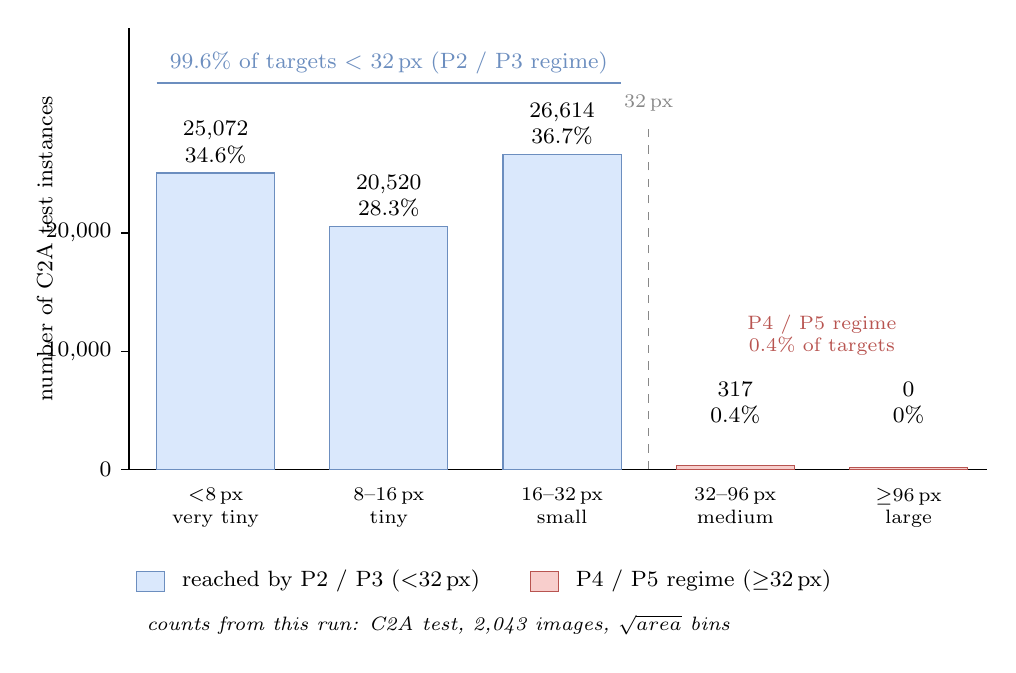
\begin{tikzpicture}[font=\footnotesize]
  % ---- axes ----
  \draw[black] (0.9,0) -- (0.9,5.6);
  \draw[black] (0.9,0) -- (11.8,0);
  \foreach \c/\y in {0/0, 10{,}000/1.5, 20{,}000/3.0}{%
    \draw[black] (0.8,\y) -- (0.9,\y);
    \node[left] at (0.8,\y) {\c};
  }
  \node[rotate=90,anchor=south] at (0.05,2.8) {number of C2A test instances};

  % ---- 32 px boundary (between small and medium) ----
  \draw[sdGrey,dashed] (7.5,0) -- (7.5,4.4);
  \node[sdGrey,font=\scriptsize,anchor=south] at (7.5,4.42) {32\,px};

  % ---- bars: blue (<32 px, P2/P3 regime), red (>=32 px, P4/P5 regime) ----
  \filldraw[fill=sdBlueFill,draw=sdBlueStroke] (1.25,0) rectangle (2.75,3.7608);
  \filldraw[fill=sdBlueFill,draw=sdBlueStroke] (3.45,0) rectangle (4.95,3.0780);
  \filldraw[fill=sdBlueFill,draw=sdBlueStroke] (5.65,0) rectangle (7.15,3.9921);
  \filldraw[fill=sdRedFill,draw=sdRedStroke]   (7.85,0) rectangle (9.35,0.0476);
  \filldraw[fill=sdRedFill,draw=sdRedStroke]   (10.05,0) rectangle (11.55,0.02);

  % ---- count + percent above each bar ----
  \node[above,align=center] at (2.0,3.7608) {25{,}072\\34.6\%};
  \node[above,align=center] at (4.2,3.0780) {20{,}520\\28.3\%};
  \node[above,align=center] at (6.4,3.9921) {26{,}614\\36.7\%};
  \node[above,align=center] at (8.6,0.45)   {317\\0.4\%};
  \node[above,align=center] at (10.8,0.45)  {0\\0\%};

  % ---- x labels: size range + class ----
  \node[below,align=center,font=\scriptsize] at (2.0,-0.12)  {$<$8\,px\\very tiny};
  \node[below,align=center,font=\scriptsize] at (4.2,-0.12)  {8--16\,px\\tiny};
  \node[below,align=center,font=\scriptsize] at (6.4,-0.12)  {16--32\,px\\small};
  \node[below,align=center,font=\scriptsize] at (8.6,-0.12)  {32--96\,px\\medium};
  \node[below,align=center,font=\scriptsize] at (10.8,-0.12) {$\geq$96\,px\\large};

  % ---- annotations ----
  \draw[sdBlueStroke,thick] (1.25,4.9) -- (7.15,4.9);
  \node[above,text=sdBlueStroke] at (4.2,4.9) {99.6\% of targets $<$ 32\,px  (P2 / P3 regime)};
  \node[align=center,text=sdRedStroke,font=\scriptsize] at (9.7,1.7) {P4 / P5 regime\\0.4\% of targets};

  % ---- legend ----
  \filldraw[fill=sdBlueFill,draw=sdBlueStroke] (1.0,-1.55) rectangle (1.35,-1.30);
  \node[anchor=west] at (1.45,-1.425) {reached by P2 / P3 ($<$32\,px)};
  \filldraw[fill=sdRedFill,draw=sdRedStroke] (6.0,-1.55) rectangle (6.35,-1.30);
  \node[anchor=west] at (6.45,-1.425) {P4 / P5 regime ($\geq$32\,px)};
  \node[anchor=west,font=\itshape\scriptsize] at (1.0,-1.98)
        {counts from this run: C2A test, 2{,}043 images, $\sqrt{\text{area}}$ bins};
\end{tikzpicture}

%  y = count * 0.00015 cm   (20,000 instances -> 3 cm)
% ============================================================================
\definecolor{sdBlueFill}{HTML}{DAE8FC}
\definecolor{sdBlueStroke}{HTML}{6C8EBF}
\definecolor{sdRedFill}{HTML}{F8CECC}
\definecolor{sdRedStroke}{HTML}{B85450}
\definecolor{sdGrey}{HTML}{888888}
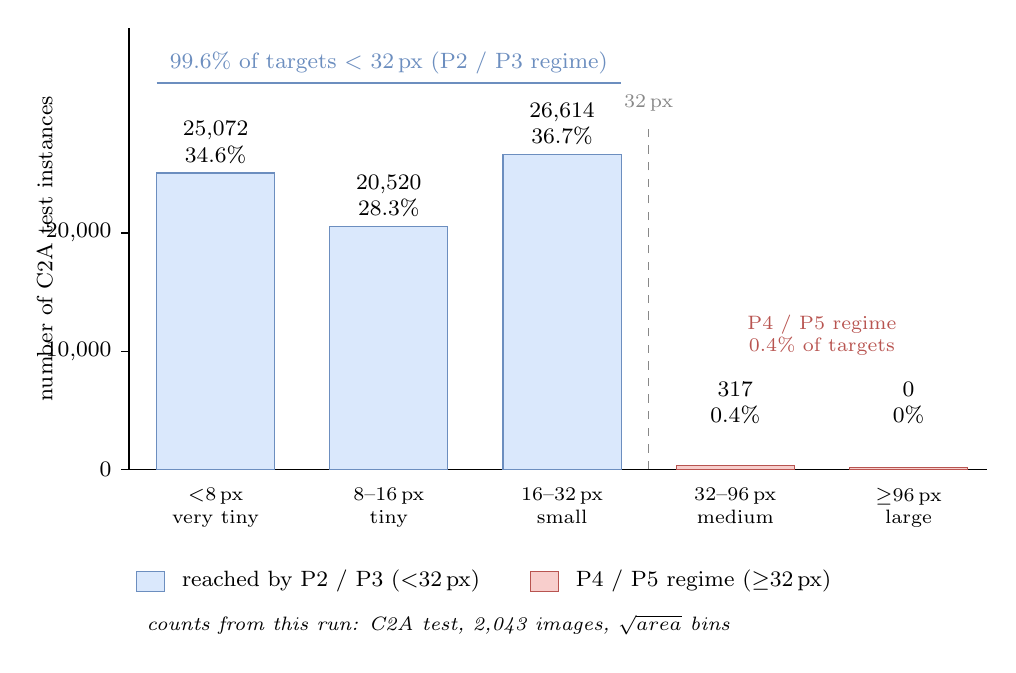
\begin{tikzpicture}[font=\footnotesize]
  % ---- axes ----
  \draw[black] (0.9,0) -- (0.9,5.6);
  \draw[black] (0.9,0) -- (11.8,0);
  \foreach \c/\y in {0/0, 10{,}000/1.5, 20{,}000/3.0}{%
    \draw[black] (0.8,\y) -- (0.9,\y);
    \node[left] at (0.8,\y) {\c};
  }
  \node[rotate=90,anchor=south] at (0.05,2.8) {number of C2A test instances};

  % ---- 32 px boundary (between small and medium) ----
  \draw[sdGrey,dashed] (7.5,0) -- (7.5,4.4);
  \node[sdGrey,font=\scriptsize,anchor=south] at (7.5,4.42) {32\,px};

  % ---- bars: blue (<32 px, P2/P3 regime), red (>=32 px, P4/P5 regime) ----
  \filldraw[fill=sdBlueFill,draw=sdBlueStroke] (1.25,0) rectangle (2.75,3.7608);
  \filldraw[fill=sdBlueFill,draw=sdBlueStroke] (3.45,0) rectangle (4.95,3.0780);
  \filldraw[fill=sdBlueFill,draw=sdBlueStroke] (5.65,0) rectangle (7.15,3.9921);
  \filldraw[fill=sdRedFill,draw=sdRedStroke]   (7.85,0) rectangle (9.35,0.0476);
  \filldraw[fill=sdRedFill,draw=sdRedStroke]   (10.05,0) rectangle (11.55,0.02);

  % ---- count + percent above each bar ----
  \node[above,align=center] at (2.0,3.7608) {25{,}072\\34.6\%};
  \node[above,align=center] at (4.2,3.0780) {20{,}520\\28.3\%};
  \node[above,align=center] at (6.4,3.9921) {26{,}614\\36.7\%};
  \node[above,align=center] at (8.6,0.45)   {317\\0.4\%};
  \node[above,align=center] at (10.8,0.45)  {0\\0\%};

  % ---- x labels: size range + class ----
  \node[below,align=center,font=\scriptsize] at (2.0,-0.12)  {$<$8\,px\\very tiny};
  \node[below,align=center,font=\scriptsize] at (4.2,-0.12)  {8--16\,px\\tiny};
  \node[below,align=center,font=\scriptsize] at (6.4,-0.12)  {16--32\,px\\small};
  \node[below,align=center,font=\scriptsize] at (8.6,-0.12)  {32--96\,px\\medium};
  \node[below,align=center,font=\scriptsize] at (10.8,-0.12) {$\geq$96\,px\\large};

  % ---- annotations ----
  \draw[sdBlueStroke,thick] (1.25,4.9) -- (7.15,4.9);
  \node[above,text=sdBlueStroke] at (4.2,4.9) {99.6\% of targets $<$ 32\,px  (P2 / P3 regime)};
  \node[align=center,text=sdRedStroke,font=\scriptsize] at (9.7,1.7) {P4 / P5 regime\\0.4\% of targets};

  % ---- legend ----
  \filldraw[fill=sdBlueFill,draw=sdBlueStroke] (1.0,-1.55) rectangle (1.35,-1.30);
  \node[anchor=west] at (1.45,-1.425) {reached by P2 / P3 ($<$32\,px)};
  \filldraw[fill=sdRedFill,draw=sdRedStroke] (6.0,-1.55) rectangle (6.35,-1.30);
  \node[anchor=west] at (6.45,-1.425) {P4 / P5 regime ($\geq$32\,px)};
  \node[anchor=west,font=\itshape\scriptsize] at (1.0,-1.98)
        {counts from this run: C2A test, 2{,}043 images, $\sqrt{\text{area}}$ bins};
\end{tikzpicture}

%  y = count * 0.00015 cm   (20,000 instances -> 3 cm)
% ============================================================================
\definecolor{sdBlueFill}{HTML}{DAE8FC}
\definecolor{sdBlueStroke}{HTML}{6C8EBF}
\definecolor{sdRedFill}{HTML}{F8CECC}
\definecolor{sdRedStroke}{HTML}{B85450}
\definecolor{sdGrey}{HTML}{888888}
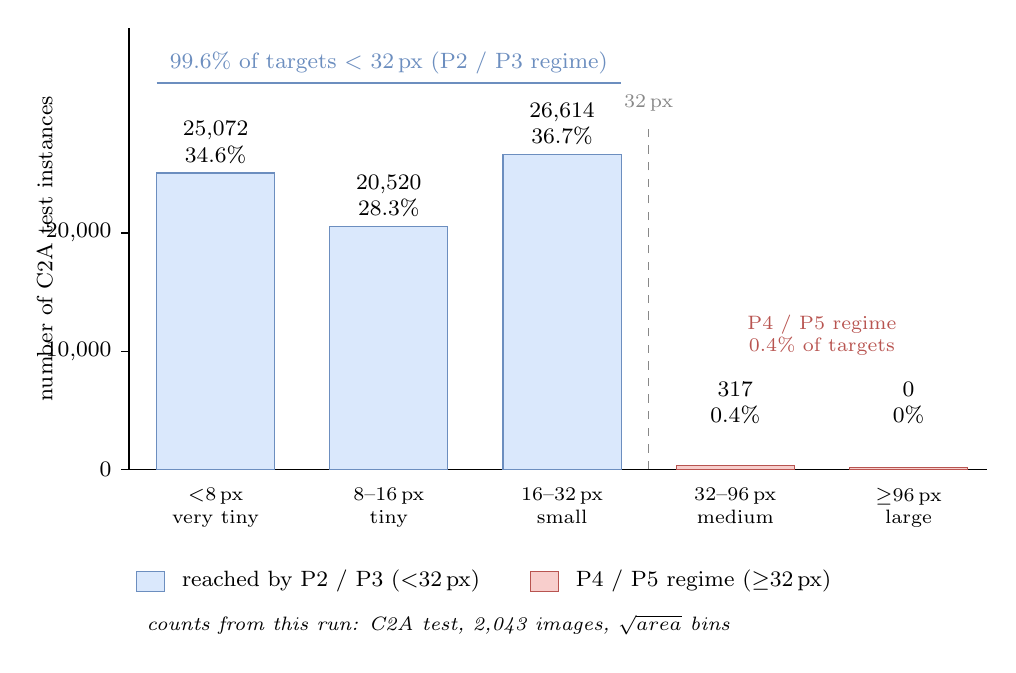
\begin{tikzpicture}[font=\footnotesize]
  % ---- axes ----
  \draw[black] (0.9,0) -- (0.9,5.6);
  \draw[black] (0.9,0) -- (11.8,0);
  \foreach \c/\y in {0/0, 10{,}000/1.5, 20{,}000/3.0}{%
    \draw[black] (0.8,\y) -- (0.9,\y);
    \node[left] at (0.8,\y) {\c};
  }
  \node[rotate=90,anchor=south] at (0.05,2.8) {number of C2A test instances};

  % ---- 32 px boundary (between small and medium) ----
  \draw[sdGrey,dashed] (7.5,0) -- (7.5,4.4);
  \node[sdGrey,font=\scriptsize,anchor=south] at (7.5,4.42) {32\,px};

  % ---- bars: blue (<32 px, P2/P3 regime), red (>=32 px, P4/P5 regime) ----
  \filldraw[fill=sdBlueFill,draw=sdBlueStroke] (1.25,0) rectangle (2.75,3.7608);
  \filldraw[fill=sdBlueFill,draw=sdBlueStroke] (3.45,0) rectangle (4.95,3.0780);
  \filldraw[fill=sdBlueFill,draw=sdBlueStroke] (5.65,0) rectangle (7.15,3.9921);
  \filldraw[fill=sdRedFill,draw=sdRedStroke]   (7.85,0) rectangle (9.35,0.0476);
  \filldraw[fill=sdRedFill,draw=sdRedStroke]   (10.05,0) rectangle (11.55,0.02);

  % ---- count + percent above each bar ----
  \node[above,align=center] at (2.0,3.7608) {25{,}072\\34.6\%};
  \node[above,align=center] at (4.2,3.0780) {20{,}520\\28.3\%};
  \node[above,align=center] at (6.4,3.9921) {26{,}614\\36.7\%};
  \node[above,align=center] at (8.6,0.45)   {317\\0.4\%};
  \node[above,align=center] at (10.8,0.45)  {0\\0\%};

  % ---- x labels: size range + class ----
  \node[below,align=center,font=\scriptsize] at (2.0,-0.12)  {$<$8\,px\\very tiny};
  \node[below,align=center,font=\scriptsize] at (4.2,-0.12)  {8--16\,px\\tiny};
  \node[below,align=center,font=\scriptsize] at (6.4,-0.12)  {16--32\,px\\small};
  \node[below,align=center,font=\scriptsize] at (8.6,-0.12)  {32--96\,px\\medium};
  \node[below,align=center,font=\scriptsize] at (10.8,-0.12) {$\geq$96\,px\\large};

  % ---- annotations ----
  \draw[sdBlueStroke,thick] (1.25,4.9) -- (7.15,4.9);
  \node[above,text=sdBlueStroke] at (4.2,4.9) {99.6\% of targets $<$ 32\,px  (P2 / P3 regime)};
  \node[align=center,text=sdRedStroke,font=\scriptsize] at (9.7,1.7) {P4 / P5 regime\\0.4\% of targets};

  % ---- legend ----
  \filldraw[fill=sdBlueFill,draw=sdBlueStroke] (1.0,-1.55) rectangle (1.35,-1.30);
  \node[anchor=west] at (1.45,-1.425) {reached by P2 / P3 ($<$32\,px)};
  \filldraw[fill=sdRedFill,draw=sdRedStroke] (6.0,-1.55) rectangle (6.35,-1.30);
  \node[anchor=west] at (6.45,-1.425) {P4 / P5 regime ($\geq$32\,px)};
  \node[anchor=west,font=\itshape\scriptsize] at (1.0,-1.98)
        {counts from this run: C2A test, 2{,}043 images, $\sqrt{\text{area}}$ bins};
\end{tikzpicture}

%  y = count * 0.00015 cm   (20,000 instances -> 3 cm)
% ============================================================================
\definecolor{sdBlueFill}{HTML}{DAE8FC}
\definecolor{sdBlueStroke}{HTML}{6C8EBF}
\definecolor{sdRedFill}{HTML}{F8CECC}
\definecolor{sdRedStroke}{HTML}{B85450}
\definecolor{sdGrey}{HTML}{888888}
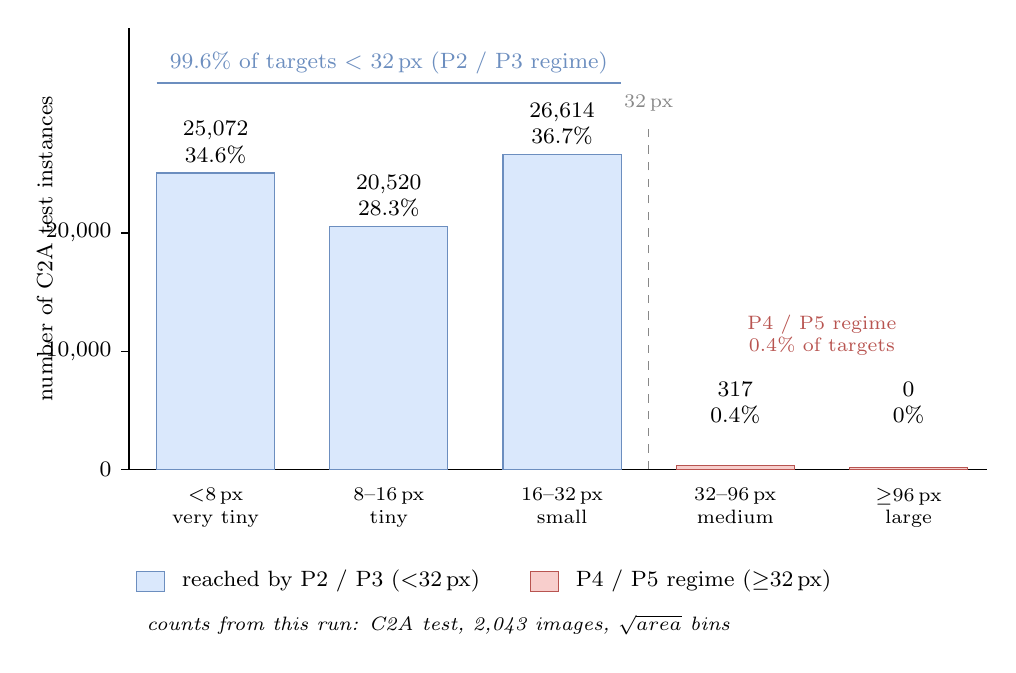
\begin{tikzpicture}[font=\footnotesize]
  % ---- axes ----
  \draw[black] (0.9,0) -- (0.9,5.6);
  \draw[black] (0.9,0) -- (11.8,0);
  \foreach \c/\y in {0/0, 10{,}000/1.5, 20{,}000/3.0}{%
    \draw[black] (0.8,\y) -- (0.9,\y);
    \node[left] at (0.8,\y) {\c};
  }
  \node[rotate=90,anchor=south] at (0.05,2.8) {number of C2A test instances};

  % ---- 32 px boundary (between small and medium) ----
  \draw[sdGrey,dashed] (7.5,0) -- (7.5,4.4);
  \node[sdGrey,font=\scriptsize,anchor=south] at (7.5,4.42) {32\,px};

  % ---- bars: blue (<32 px, P2/P3 regime), red (>=32 px, P4/P5 regime) ----
  \filldraw[fill=sdBlueFill,draw=sdBlueStroke] (1.25,0) rectangle (2.75,3.7608);
  \filldraw[fill=sdBlueFill,draw=sdBlueStroke] (3.45,0) rectangle (4.95,3.0780);
  \filldraw[fill=sdBlueFill,draw=sdBlueStroke] (5.65,0) rectangle (7.15,3.9921);
  \filldraw[fill=sdRedFill,draw=sdRedStroke]   (7.85,0) rectangle (9.35,0.0476);
  \filldraw[fill=sdRedFill,draw=sdRedStroke]   (10.05,0) rectangle (11.55,0.02);

  % ---- count + percent above each bar ----
  \node[above,align=center] at (2.0,3.7608) {25{,}072\\34.6\%};
  \node[above,align=center] at (4.2,3.0780) {20{,}520\\28.3\%};
  \node[above,align=center] at (6.4,3.9921) {26{,}614\\36.7\%};
  \node[above,align=center] at (8.6,0.45)   {317\\0.4\%};
  \node[above,align=center] at (10.8,0.45)  {0\\0\%};

  % ---- x labels: size range + class ----
  \node[below,align=center,font=\scriptsize] at (2.0,-0.12)  {$<$8\,px\\very tiny};
  \node[below,align=center,font=\scriptsize] at (4.2,-0.12)  {8--16\,px\\tiny};
  \node[below,align=center,font=\scriptsize] at (6.4,-0.12)  {16--32\,px\\small};
  \node[below,align=center,font=\scriptsize] at (8.6,-0.12)  {32--96\,px\\medium};
  \node[below,align=center,font=\scriptsize] at (10.8,-0.12) {$\geq$96\,px\\large};

  % ---- annotations ----
  \draw[sdBlueStroke,thick] (1.25,4.9) -- (7.15,4.9);
  \node[above,text=sdBlueStroke] at (4.2,4.9) {99.6\% of targets $<$ 32\,px  (P2 / P3 regime)};
  \node[align=center,text=sdRedStroke,font=\scriptsize] at (9.7,1.7) {P4 / P5 regime\\0.4\% of targets};

  % ---- legend ----
  \filldraw[fill=sdBlueFill,draw=sdBlueStroke] (1.0,-1.55) rectangle (1.35,-1.30);
  \node[anchor=west] at (1.45,-1.425) {reached by P2 / P3 ($<$32\,px)};
  \filldraw[fill=sdRedFill,draw=sdRedStroke] (6.0,-1.55) rectangle (6.35,-1.30);
  \node[anchor=west] at (6.45,-1.425) {P4 / P5 regime ($\geq$32\,px)};
  \node[anchor=west,font=\itshape\scriptsize] at (1.0,-1.98)
        {counts from this run: C2A test, 2{,}043 images, $\sqrt{\text{area}}$ bins};
\end{tikzpicture}
